\documentclass{standalone}
\usepackage{tikz}
\usetikzlibrary{patterns, positioning}

\begin{document}
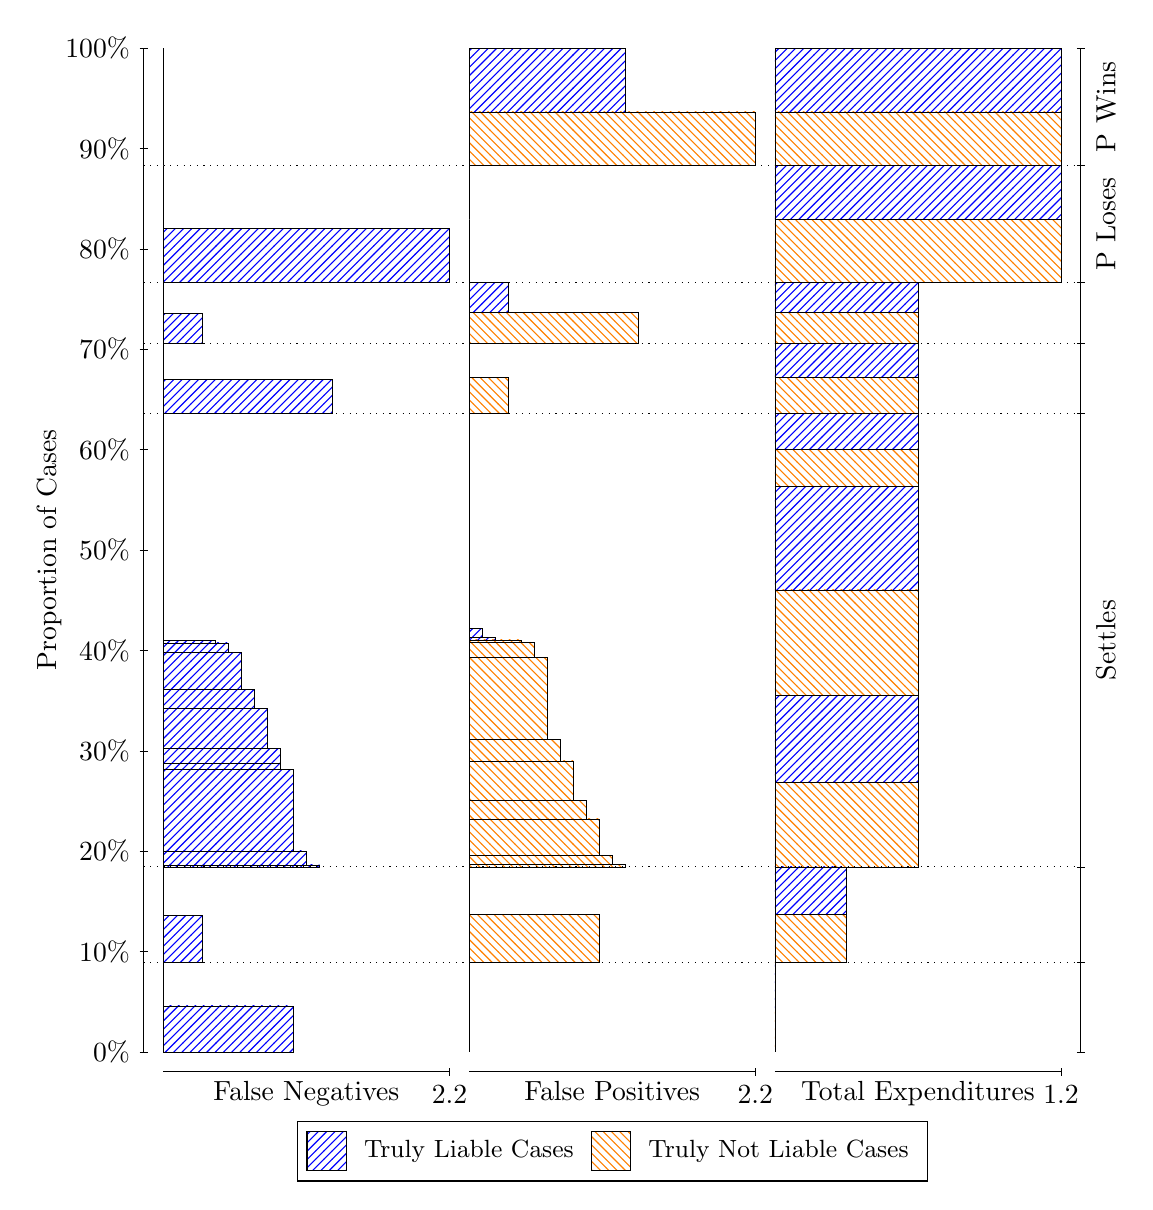
\begin{tikzpicture}
\draw[black, very thin] (1.5,1.75) -- (1.5,14.5);
\node[rotate=90, anchor=center] at (0.3, 8.125) {Proportion of Cases};
\draw[black, very thin] (1.45,1.75) -- (1.55,1.75);
\node[anchor=east] at (1.45, 1.75) {0\%};
\draw[black, very thin] (1.45,3.025) -- (1.55,3.025);
\node[anchor=east] at (1.45, 3.025) {10\%};
\draw[black, very thin] (1.45,4.3) -- (1.55,4.3);
\node[anchor=east] at (1.45, 4.3) {20\%};
\draw[black, very thin] (1.45,5.575) -- (1.55,5.575);
\node[anchor=east] at (1.45, 5.575) {30\%};
\draw[black, very thin] (1.45,6.85) -- (1.55,6.85);
\node[anchor=east] at (1.45, 6.85) {40\%};
\draw[black, very thin] (1.45,8.125) -- (1.55,8.125);
\node[anchor=east] at (1.45, 8.125) {50\%};
\draw[black, very thin] (1.45,9.4) -- (1.55,9.4);
\node[anchor=east] at (1.45, 9.4) {60\%};
\draw[black, very thin] (1.45,10.675) -- (1.55,10.675);
\node[anchor=east] at (1.45, 10.675) {70\%};
\draw[black, very thin] (1.45,11.95) -- (1.55,11.95);
\node[anchor=east] at (1.45, 11.95) {80\%};
\draw[black, very thin] (1.45,13.225) -- (1.55,13.225);
\node[anchor=east] at (1.45, 13.225) {90\%};
\draw[black, very thin] (1.45,14.5) -- (1.55,14.5);
\node[anchor=east] at (1.45, 14.5) {100\%};

\draw[black, very thin] (13.4,1.75) -- (13.4,14.5);
\draw[black, very thin] (13.35,1.75) -- (13.45,1.75);
\node[anchor=west] at (13.35, 1.75) {};
\draw[black, very thin] (13.35,2.8833) -- (13.45,2.8833);
\node[anchor=west] at (13.35, 2.8833) {};
\draw[black, very thin] (13.35,4.1008) -- (13.45,4.1008);
\node[anchor=west] at (13.35, 4.1008) {};
\draw[black, very thin] (13.35,9.861) -- (13.45,9.861);
\node[anchor=west] at (13.35, 9.861) {};
\draw[black, very thin] (13.35,10.749) -- (13.45,10.749);
\node[anchor=west] at (13.35, 10.749) {};
\draw[black, very thin] (13.35,11.52) -- (13.45,11.52);
\node[anchor=west] at (13.35, 11.52) {};
\draw[black, very thin] (13.35,13.008) -- (13.45,13.008);
\node[anchor=west] at (13.35, 13.008) {};
\draw[black, very thin] (13.35,14.5) -- (13.45,14.5);
\node[anchor=west] at (13.35, 14.5) {};

\draw[black, very thin, pattern color=blue, pattern=north east lines] (1.75,1.75) rectangle (3.4015,2.3355);
\draw[black, very thin, pattern color=orange, pattern=north west lines] (1.75,2.3355) rectangle (1.75,2.8833);
\draw[black, very thin, pattern color=blue, pattern=north east lines] (1.75,2.8833) rectangle (2.2455,3.4826);
\draw[black, very thin, pattern color=orange, pattern=north west lines] (1.75,3.4826) rectangle (1.75,4.1008);
\draw[black, very thin, pattern color=blue, pattern=north east lines] (1.75,4.1008) rectangle (3.7318,4.1254);
\draw[black, very thin, pattern color=blue, pattern=north east lines] (1.75,4.1254) rectangle (3.5667,4.3026);
\draw[black, very thin, pattern color=blue, pattern=north east lines] (1.75,4.3026) rectangle (3.4015,5.3436);
\draw[black, very thin, pattern color=blue, pattern=north east lines] (1.75,5.3436) rectangle (3.2364,5.4199);
\draw[black, very thin, pattern color=blue, pattern=north east lines] (1.75,5.4199) rectangle (3.2364,5.6094);
\draw[black, very thin, pattern color=blue, pattern=north east lines] (1.75,5.6094) rectangle (3.0712,6.1172);
\draw[black, very thin, pattern color=blue, pattern=north east lines] (1.75,6.1172) rectangle (2.9061,6.356);
\draw[black, very thin, pattern color=blue, pattern=north east lines] (1.75,6.356) rectangle (2.7409,6.8286);
\draw[black, very thin, pattern color=blue, pattern=north east lines] (1.75,6.8286) rectangle (2.5758,6.9467);
\draw[black, very thin, pattern color=blue, pattern=north east lines] (1.75,6.9467) rectangle (2.4106,6.9793);
\draw[black, very thin, pattern color=orange, pattern=north west lines] (1.75,6.9793) rectangle (1.75,9.861);
\draw[black, very thin, pattern color=blue, pattern=north east lines] (1.75,9.861) rectangle (3.897,10.294);
\draw[black, very thin, pattern color=orange, pattern=north west lines] (1.75,10.294) rectangle (1.75,10.749);
\draw[black, very thin, pattern color=blue, pattern=north east lines] (1.75,10.749) rectangle (2.2455,11.127);
\draw[black, very thin, pattern color=orange, pattern=north west lines] (1.75,11.127) rectangle (1.75,11.52);
\draw[black, very thin, pattern color=blue, pattern=north east lines] (1.75,11.52) rectangle (5.3833,12.209);
\draw[black, very thin, pattern color=orange, pattern=north west lines] (1.75,12.209) rectangle (1.75,13.008);
\draw[black, very thin, pattern color=orange, pattern=north west lines] (1.75,13.008) rectangle (1.75,13.688);
\draw[black, very thin, pattern color=blue, pattern=north east lines] (1.75,13.688) rectangle (1.75,14.5);
\draw[black, very thin, pattern color=orange, pattern=north west lines] (5.6333,1.75) rectangle (5.6333,2.2978);
\draw[black, very thin, pattern color=blue, pattern=north east lines] (5.6333,2.2978) rectangle (5.6333,2.8833);
\draw[black, very thin, pattern color=orange, pattern=north west lines] (5.6333,2.8833) rectangle (7.2848,3.5015);
\draw[black, very thin, pattern color=blue, pattern=north east lines] (5.6333,3.5015) rectangle (5.6333,4.1008);
\draw[black, very thin, pattern color=orange, pattern=north west lines] (5.6333,4.1008) rectangle (7.6152,4.1339);
\draw[black, very thin, pattern color=orange, pattern=north west lines] (5.6333,4.1339) rectangle (7.45,4.2494);
\draw[black, very thin, pattern color=orange, pattern=north west lines] (5.6333,4.2494) rectangle (7.2848,4.7095);
\draw[black, very thin, pattern color=orange, pattern=north west lines] (5.6333,4.7095) rectangle (7.1197,4.9454);
\draw[black, very thin, pattern color=orange, pattern=north west lines] (5.6333,4.9454) rectangle (6.9545,5.4479);
\draw[black, very thin, pattern color=orange, pattern=north west lines] (5.6333,5.4479) rectangle (6.7894,5.723);
\draw[black, very thin, pattern color=orange, pattern=north west lines] (5.6333,5.723) rectangle (6.6242,6.7651);
\draw[black, very thin, pattern color=orange, pattern=north west lines] (5.6333,6.7651) rectangle (6.4591,6.9554);
\draw[black, very thin, pattern color=orange, pattern=north west lines] (5.6333,6.9554) rectangle (6.2939,6.9826);
\draw[black, very thin, pattern color=blue, pattern=north east lines] (5.6333,6.9826) rectangle (5.9636,7.0152);
\draw[black, very thin, pattern color=blue, pattern=north east lines] (5.6333,7.0152) rectangle (5.7985,7.1333);
\draw[black, very thin, pattern color=blue, pattern=north east lines] (5.6333,7.1333) rectangle (5.6333,9.861);
\draw[black, very thin, pattern color=orange, pattern=north west lines] (5.6333,9.861) rectangle (6.1288,10.316);
\draw[black, very thin, pattern color=blue, pattern=north east lines] (5.6333,10.316) rectangle (5.6333,10.749);
\draw[black, very thin, pattern color=orange, pattern=north west lines] (5.6333,10.749) rectangle (7.7803,11.142);
\draw[black, very thin, pattern color=blue, pattern=north east lines] (5.6333,11.142) rectangle (6.1288,11.52);
\draw[black, very thin, pattern color=orange, pattern=north west lines] (5.6333,11.52) rectangle (5.6333,12.32);
\draw[black, very thin, pattern color=blue, pattern=north east lines] (5.6333,12.32) rectangle (5.6333,13.008);
\draw[black, very thin, pattern color=orange, pattern=north west lines] (5.6333,13.008) rectangle (9.2667,13.688);
\draw[black, very thin, pattern color=blue, pattern=north east lines] (5.6333,13.688) rectangle (7.6152,14.5);
\draw[black, very thin, pattern color=orange, pattern=north west lines] (9.5167,1.75) rectangle (9.5167,2.2978);
\draw[black, very thin, pattern color=blue, pattern=north east lines] (9.5167,2.2978) rectangle (9.5167,2.8833);
\draw[black, very thin, pattern color=orange, pattern=north west lines] (9.5167,2.8833) rectangle (10.425,3.5015);
\draw[black, very thin, pattern color=blue, pattern=north east lines] (9.5167,3.5015) rectangle (10.425,4.1008);
\draw[black, very thin, pattern color=orange, pattern=north west lines] (9.5167,4.1008) rectangle (11.333,5.179);
\draw[black, very thin, pattern color=blue, pattern=north east lines] (9.5167,5.179) rectangle (11.333,6.2775);
\draw[black, very thin, pattern color=orange, pattern=north west lines] (9.5167,6.2775) rectangle (11.333,7.6176);
\draw[black, very thin, pattern color=blue, pattern=north east lines] (9.5167,7.6176) rectangle (11.333,8.9367);
\draw[black, very thin, pattern color=orange, pattern=north west lines] (9.5167,8.9367) rectangle (11.333,9.4002);
\draw[black, very thin, pattern color=blue, pattern=north east lines] (9.5167,9.4002) rectangle (11.333,9.861);
\draw[black, very thin, pattern color=orange, pattern=north west lines] (9.5167,9.861) rectangle (11.333,10.316);
\draw[black, very thin, pattern color=blue, pattern=north east lines] (9.5167,10.316) rectangle (11.333,10.749);
\draw[black, very thin, pattern color=orange, pattern=north west lines] (9.5167,10.749) rectangle (11.333,11.142);
\draw[black, very thin, pattern color=blue, pattern=north east lines] (9.5167,11.142) rectangle (11.333,11.52);
\draw[black, very thin, pattern color=orange, pattern=north west lines] (9.5167,11.52) rectangle (13.15,12.32);
\draw[black, very thin, pattern color=blue, pattern=north east lines] (9.5167,12.32) rectangle (13.15,13.008);
\draw[black, very thin, pattern color=orange, pattern=north west lines] (9.5167,13.008) rectangle (13.15,13.688);
\draw[black, very thin, pattern color=blue, pattern=north east lines] (9.5167,13.688) rectangle (13.15,14.5);
\draw[black, dotted] (1.5,2.8833) -- (13.4,2.8833);
\draw[black, dotted] (1.5,4.1008) -- (13.4,4.1008);
\draw[black, dotted] (1.5,9.861) -- (13.4,9.861);
\draw[black, dotted] (1.5,10.749) -- (13.4,10.749);
\draw[black, dotted] (1.5,11.52) -- (13.4,11.52);
\draw[black, dotted] (1.5,13.008) -- (13.4,13.008);
\draw[black, very thin] (1.75,1.5) -- (5.3833,1.5);
\node[anchor=north] at (3.5667, 1.5) {False Negatives};
\draw[black, very thin] (5.3833,1.45) -- (5.3833,1.55);
\node[anchor=north] at (5.3833, 1.45) {2.2};

\draw[black, very thin] (5.6333,1.5) -- (9.2667,1.5);
\node[anchor=north] at (7.45, 1.5) {False Positives};
\draw[black, very thin] (9.2667,1.45) -- (9.2667,1.55);
\node[anchor=north] at (9.2667, 1.45) {2.2};

\draw[black, very thin] (9.5167,1.5) -- (13.15,1.5);
\node[anchor=north] at (11.333, 1.5) {Total Expenditures};
\draw[black, very thin] (13.15,1.45) -- (13.15,1.55);
\node[anchor=north] at (13.15, 1.45) {1.2};



\node[black, centered, rotate=90] at (13.72, 6.9809) {Settles};


\node[black, centered, rotate=90] at (13.72, 12.264) {P Loses};
\node[black, centered, rotate=90] at (13.72, 13.754) {P Wins};

\draw (7.449999999999999,1.5) node[draw=none] (baseCoordinate) {};
\begin{scope}[align=center]
        \matrix[scale=0.5, draw=black, below=0.5cm of baseCoordinate, nodes={draw}, column sep=0.1cm]{
            \node[rectangle, draw, minimum width=0.5cm, minimum height=0.5cm, pattern=north east lines, pattern color=blue] {}; &
            \node[draw=none, font=\small] (B) {Truly Liable Cases}; &
            \node[rectangle, draw, minimum width=0.5cm, minimum height=0.5cm, pattern=north west lines, pattern color=orange] {}; &
            \node[draw=none, font=\small] (B) {Truly Not Liable Cases}; \\
            };
\end{scope}

\end{tikzpicture}
\end{document}